% !TEX TS-program = pdflatex
% !TEX encoding = UTF-8 Unicode

% This is a simple template for a LaTeX document using the "article" class.
% See "book", "report", "letter" for other types of document.

\documentclass[11pt]{article} % use larger type; default would be 10pt

\usepackage[utf8]{inputenc} % set input encoding (not needed with XeLaTeX)

%%% Examples of Article customizations
% These packages are optional, depending whether you want the features they provide.
% See the LaTeX Companion or other references for full information.

%%% PAGE DIMENSIONS
\usepackage{geometry} % to change the page dimensions
\geometry{a4paper} % or letterpaper (US) or a5paper or....
% \geometry{margin=2in} % for example, change the margins to 2 inches all round
% \geometry{landscape} % set up the page for landscape
%   read geometry.pdf for detailed page layout information

\usepackage{graphicx} % support the \includegraphics command and options

\usepackage{listings}
\usepackage{color}
\usepackage{courier}
% \usepackage[parfill]{parskip} % Activate to begin paragraphs with an empty line rather than an indent

%%% PACKAGES
\usepackage[table]{xcolor}
\usepackage{booktabs} % for much better looking tables
\usepackage{array} % for better arrays (eg matrices) in maths
\usepackage{paralist} % very flexible & customisable lists (eg. enumerate/itemize, etc.)
\usepackage{verbatim} % adds environment for commenting out blocks of text & for better verbatim
\usepackage{subfig} % make it possible to include more than one captioned figure/table in a single float
\usepackage{amsmath, mathtools}
\usepackage{graphicx}
% These packages are all incorporated in the memoir class to one degree or another...

%%% HEADERS & FOOTERS
\usepackage{fancyhdr} % This should be set AFTER setting up the page geometry
\pagestyle{fancy} % options: empty , plain , fancy
\renewcommand{\headrulewidth}{0pt} % customise the layout...
\lhead{}\chead{}\rhead{}
\lfoot{}\cfoot{\thepage}\rfoot{}

%%% SECTION TITLE APPEARANCE
\usepackage{sectsty}
\allsectionsfont{\sffamily\mdseries\upshape} % (See the fntguide.pdf for font help)
% (This matches ConTeXt defaults)

%%% ToC (table of contents) APPEARANCE
\usepackage[nottoc,notlof,notlot]{tocbibind} % Put the bibliography in the ToC
\usepackage[titles,subfigure]{tocloft} % Alter the style of the Table of Contents
\renewcommand{\cftsecfont}{\rmfamily\mdseries\upshape}
\renewcommand{\cftsecpagefont}{\rmfamily\mdseries\upshape} % No bold!

\definecolor{codegray}{rgb}{0.5,0.5,0.5}
\definecolor{codered}{rgb}{0.85,0.27,0.32}
\definecolor{codeorange}{rgb}{0.96,0.45,0.0}
\lstdefinestyle{mystyle}{
    commentstyle=\color{codegray},
    keywordstyle=\bfseries,
    numberstyle=\tiny\color{codegray},
    stringstyle=\color{codered},
    basicstyle=\ttfamily,
    breaklines=true,
    captionpos=b,
    frame=single,
    keepspaces=true,
    numbers=left,
}
\lstset{style=mystyle}

%%% END Article customizations

%%% The "real" document content comes below...

\title{INF236 - Problem Set 1}
\author{Konstantin Rygol}
%\date{} % Activate to display a given date or no date (if empty),
         % otherwise the current date is printed 

\begin{document}
\maketitle

\section{General}
\subsection{Hardware}
The benchmarks were computed on ift-superbeist.klientdrift.uib.no. This is a cluster machine at the
physics institute. 
It has 48 cpu divided over 4 sockets. Each socket having one AMD Opteron(tm) Processor 6174. The
machine is quite outdated but I think I get nice benchmark/scaling results then if I run on lyng.
In the appendix you can find the output of lscpu. On this machine was much fewer traffic than on
lyng but some calculations were running anyways disturbing my benchmarks.
As the problems where quite large each program was only run once and that time taken. To ensure
better benchmark results multiple runs with the same parameters would be good to obtain statistics.

\subsection{Task 1 and 2}
Both implementation work with an arbitrary problem size. Both require the number of processes to be
even. If an uneven number of processes is given the programs will abort with a simple 
error massage.    

\section{Task 1}
%graphics
\begin{figure}[ht]
 \centering
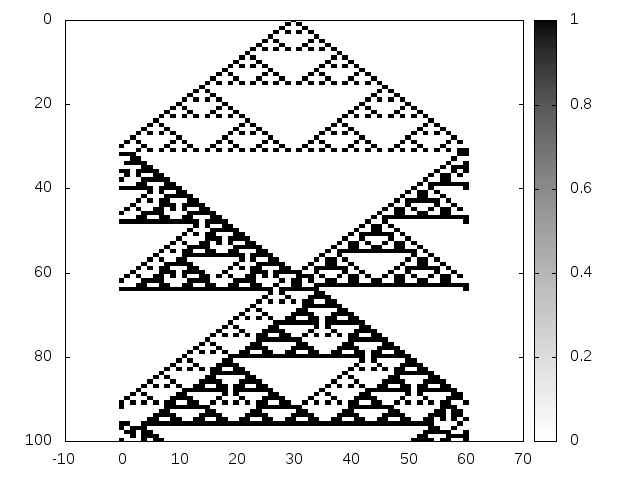
\includegraphics[width=0.8\textwidth]{graphics/Task1.png} \\
 \caption[]{100 Iterations on middle30.txt}
\end{figure}

\subsection{Algorithm}
Paralleleizig in a distributed memory system require a lot of thought on memory management. Which
variables have to be shared by all process which ones should be private. How do you divide up the
data. In this task the data stored in env (environment) will be distributed equally over p processes.
The other variables like the function will be on all ranks. 
The idea is that every rank works on its part of the environment called $env\_rank$. The ranks need 
to share the border elements so after every iteration the first and the last element are sent t
o the neighbouring ranks in a torso like fashion. After the final iteration k all env\_rank are 
gathered on rank 0 and streamed to std output. 
This kind of parallelization is highly effective as there is little communication for one iteration.
the I/O operations are all handled by rank 0. 
The biggest data transfers happens during the distribution of env and the collection of the
env\_rank.

%table
\begin{figure}
\begin{center}
\begin{tabular}{l|l|l|l|l|l|l|l|}
\hline
        & 2       & 4       & 8       & 16      & 32      & 64      & 128     \\
\hline
2048    & 0.839   & 0.667   & 0.671   & 0.945   & 1.684   & 5.158   & 27.228  \\
\hline
4096    & 1.432   & 1.136   & 0.923   & 1.180   & 1.830   & 5.751   & 31.186  \\
\hline
8096    & 2.664   & 1.856   & 1.753   & 1.544   & 2.169   & 6.603   & 31.675  \\
\hline
16384   & 4.974   & 3.689   & 2.795   & 3.018   & 2.973   & 9.071   & 35.191  \\
\hline
32768   & 9.665   & 6.902   & 5.421   & 4.604   & 5.686   & 10.830  & 41.028  \\
\hline
65536   & 19.242  & 13.402  & 11.257  & 9.446   & 8.544   & 18.510  & 49.785  \\
\hline
131072  & 38.205  & 27.354  & 21.751  & 19.074  & 18.219  & 24.236  & 64.354  \\
\hline
262144  & 75.884  & 51.557  & 42.726  & 37.375  & 34.649  & 71.878  & 110.128 \\
\hline
524288  & 152.416 & 99.968  & 79.004  & 73.948  & 68.455  & 110.441 & 415.160 \\
\hline
1048576 & 304.220 & 196.013 & 147.866 & 135.491 & 137.772 & 193.754 & 553.927 \\
\hline
2097152 & 611.076 & 385.591 & 288.120 & 244.230 & 240.036 & 340.373 & 784.973 \\
\hline
\end{tabular}
\caption{Run time in seconds of the 1d algorithm in seconds for 100000 evolutions}
\end{center}
\end{figure}


\subsection{Evaluation 1D Algorithm}
For a sufficient problem size there is a speed up with the optimum being between  p=16 and  p=32. The computation
time is linear in the input size of the starting assignment for most p. We see that for p greater
than 32 a break down in performance is observed. This is easily explained by costly synchronization.
After every iteration of the algorithm we have to synchronize therefore the speed of the whole
simulation depends on the slowest rank if we now enlarge p over the number of cores on the machine
we create some slow ranks. This is also a problem if multiple users work on one machine. 


\section{Algorithm  2d}
In this task we expanded our algorithm to a 2d model. In the way of parallelization it does not change
much. The environment is split up row wise shown in table1. Each block has length n and height n/p.
After every iteration each block send their neighbouring rows to its neighbours. This is done in a
torso like fashion.
In the folder 2-Sequential there is a python 
script generating the game\_of\_live.txt. 
To ensure that the program works the blinker figure and toad of Conan's game of life were used. 


\begin{table}
\begin{center}
\begin{tabular}{|l|c|c|r|}
  \hline
\cellcolor{blue!15}  & \cellcolor{blue!15} & \cellcolor{blue!15}  & \cellcolor{blue!15}  \\
\hline
\cellcolor{blue!15}  & \cellcolor{blue!15} & \cellcolor{blue!15}  & \cellcolor{blue!15}  \\
\hline
 \cellcolor{red!25}  & \cellcolor{red!25} & \cellcolor{red!25}  & \cellcolor{red!25}  \\
  \hline
\cellcolor{red!25}  & \cellcolor{red!25} & \cellcolor{red!25}  & \cellcolor{red!25}  \\
  \hline
\end{tabular}
\end{center}
  \caption{The table represents the data distribution scheme for the 2dCellular algorithm for 
      p = 2 and n = 4. It is a row wise decomposition of the environment}
\end{table}

\subsection{Evaluation 2d Algorithm}
The run time depends quadratic on the input size n. Which is clear as the environment consists of
$n^2$ elements. It is interesting to see that contrary to the 1d model the best number of processes
is between p=32 and p=64. This might be due to fewer iterations leading to less idle time. Some
values as the one for P=128 n=8192 might also be subject to normal fluctuations.

%Table
\begin{table}
\begin{center}
\begin{tabular}{l c|c|c|c|c|c|c|r|}
\hline
 &       & 2       & 4       & 8       & 16      & 32      & 64      & 128     \\
\hline
&1024    &118.163 &58.643  &29.596  &14.805  &7.470   &7.710   &7.477\\
\hline
&2048   &476.921 &237.184 &119.531 &59.733  &29.821  &31.148  &25.282 \\
\hline
&4096   &1928.160 &955.603 &482.584 &240.910 &121.122 &128.958 &109.26 \\
\hline
&8192   &7756.810 &3860.760 &1951.340 &973.530 &485.878 &484.671 &387.64 \\
\hline
\end{tabular}
\caption{Run time in seconds of the 2d algorithm in seconds for 1000 evolutions}
\end{center}
\end{table}

\section{Task 3}
\subsection{Algorithm branching}
The algorithm calculates a chain of associative operations and checks whether the results is in a set
F.
It takes an assignment and a branching program. The branching program defines the associative
operation. The set the operation operates on, the final set and Triplets which are the subjects to
the associative operation. We first reduce the triplets with the starting assignment to set of
elements in S that are to be "multiplied".
The idea behind and efficient parallelization is to organize the data in a
tree structure. Every rank get a share of elements that he multiplies. After it is finished it sends
its end element to rank zero that sums up all these elements to obtain the final element. 
This is allowed as the operation is associative. The limit of what we can achieve is
$\mathcal{O}(\log{m})$. 

\subsection{Proof}
It is to be shown that val(P,a) can be computed in O(log m). If we have unlimited amount of
processes p. 
Lets write down what the algorithm does:
\begin{enumerate}
\item First get $I^{1}_{a[i_1]} ... I^{m}_{a[i_m]}$
\item Calculate associative operation this takes $2*k/2$ time steps
\item Repeat step 2 until all elements are summed up 
\item Check whether final element is in F
\end{enumerate}
Now lets see where we can save time by using multi processing:
\begin{enumerate}
\item If we have m processes this can be done in linear time
\item For the second step we need $2*k/2 = k$ processes for each element to achieve linear time 
\item we have to repeat step 2 $log(m)$ times if we order the data in a tree. (Prefix sum)
\item We need r processes to do the check in linear time
\end{enumerate}
Conclusively $\mathcal{O}(\log{m})$ steps are needed if we have an unlimited amount of processes. 

\subsection{Evaluation branching}
Unfortunately my algorithm does not work correctly with the input of the branching program. I
tested it successfully earlier with another operation then the multiplication on A5. My times were
extremely short and the program now gives bad results. Therefore I could not make any meaning full
timing runs. I suspect my implementation of the A5 multiplication in my python script is corrupted.  

\section{Conclusion}
Generally the effects of parallelization became obvious. Communication was not time consuming in the
problems but synchronization is. This becomes evident for using more processes than cores. This is
also heavily influenced by other users on the same machine. For better benchmarks a scheduled system
e.g. with slurm would be beneficial. 
In the end I would say it was a nice exercise. 
\section{Appendix}

\newpage
\lstinputlisting{graphics/lscpu.txt}



\end{document}
